\chapter{Event Reconstruction} \label{chapter:reconstruction}

    \section{Introduction}

        Once a bunch-crossing event has cleared the Level 1 Trigger system, the stage of event reconstruction begins.
        An event in ATLAS is initially nothing but a collection of electrical signals emitted from the various detectors.
        Event reconstruction is the process wherein detector readings are aggregated together into meaningful patterns,
            which are interpreted as physical objects and events.
        The key objects of interest in this analysis are particle \textit{tracks} and \textit{jets}.
        As well, the way in which b-quark-initiated jets (``b-jets'') are distinguished from other jet types,
            called \textit{flavour tagging}, plays a particularly important role.
        Finally, special attention will be given to the fact that reconstruction occurs not once, but twice;
            first in the High Level Trigger online running environment,
            and again in the offline environment after events have been read out.
        The ways that reconstruction differs between these two environments plays a role
            in later stages of this analysis, and so is worth discussing.

    \FloatBarrier
    \section{Tracks} \label{sec:reco_tracks}
            
        \subsection{Track Definition}
            
            The first point of contact for anything leaving the interaction region of ATLAS is the tracking detectors.
            As such, the objects reconstructed from the tracking detectors will be the first point of discussion.
            Prior to encountering the ATLAS calorimeters,
                particles exiting the Interaction Region travel along a relatively unimpeded trajectory.
            Thanks to the inclusion of the Solenoid Magnet field encompassing the Inner Detectors,
                these trajectories reveal crucial information about the particles in an event.
            This is because any charged particle, with a momentum component orthogonal to a magnetic field,
                will trace out a \textit{helical} trajectory.
            If the shape of the helix is known, then basic electrodynamics principles can be used to determine the
                momentum and charge of the particle that formed it.
            Specifically, for a charged particle with four-momentum given as 
            \begin{equation}
            p = \minimatrix{E \\ p_T \\ \theta \\ \phi}
            \end{equation}
            the track's helical shape can reveal all components except for the energy $E$ (which will be handled by the calorimeters).
            To understand how this is achieved, one must understand how a track helix is described mathematically.
            A helix can be defined using five parameters structured in a three-dimensional parametric equation.
            There are several conventions for the form these parameters should take,
                but in ATLAS a helix is described\cite{thesis_giacinto} by a set of equations parameterised by an angle $\alpha$ as:
            \begin{equation} \begin{split}
            x(\alpha) &= x_R + d_0 \cos(\phi) + \rho \left[ \cos(\alpha) - \cos(\phi) \right] \\
            y(\alpha) &= y_R + d_0 \sin(\phi) + \rho \left[ \sin(\alpha) - \sin(\phi) \right] \\
            z(\alpha) &= z_R + z_0 - \rho \cot(\theta) (\alpha - \phi)
            \end{split} \end{equation}

            The helix is described relative to a reference point $R$,
                which is initially set to the beam-spot location in the IR.
            Later stages of tracking will redefine the equations with respect to different reference points as needed.
            The five parameters governing the shape of this helix, called \textit{perigee parameters}, 
                are described largely in terms of the ``Point of Closest Approach'' (PoCA),
                the point on the helix closest to $R$ in the $x,y$ plane.
            \begin{itemize}
                \item $d_0$: $|(x,y)|$-Distance from the origin to the closest point on the helix, in the $x,y$ plane
                \item $z_0$: $z$-Distance between the PoCA and the origin
                \item $\phi$: Angle in the $x,y$ plane of the PoCA
                \item $\theta$: The angle of the helix's trajectory in the $\rho,z$ plane
                \item $\rho$: The radius of curvature of the helix
            \end{itemize}

            \begin{figure}
                \subfloat[Perigee Parameters]{
                    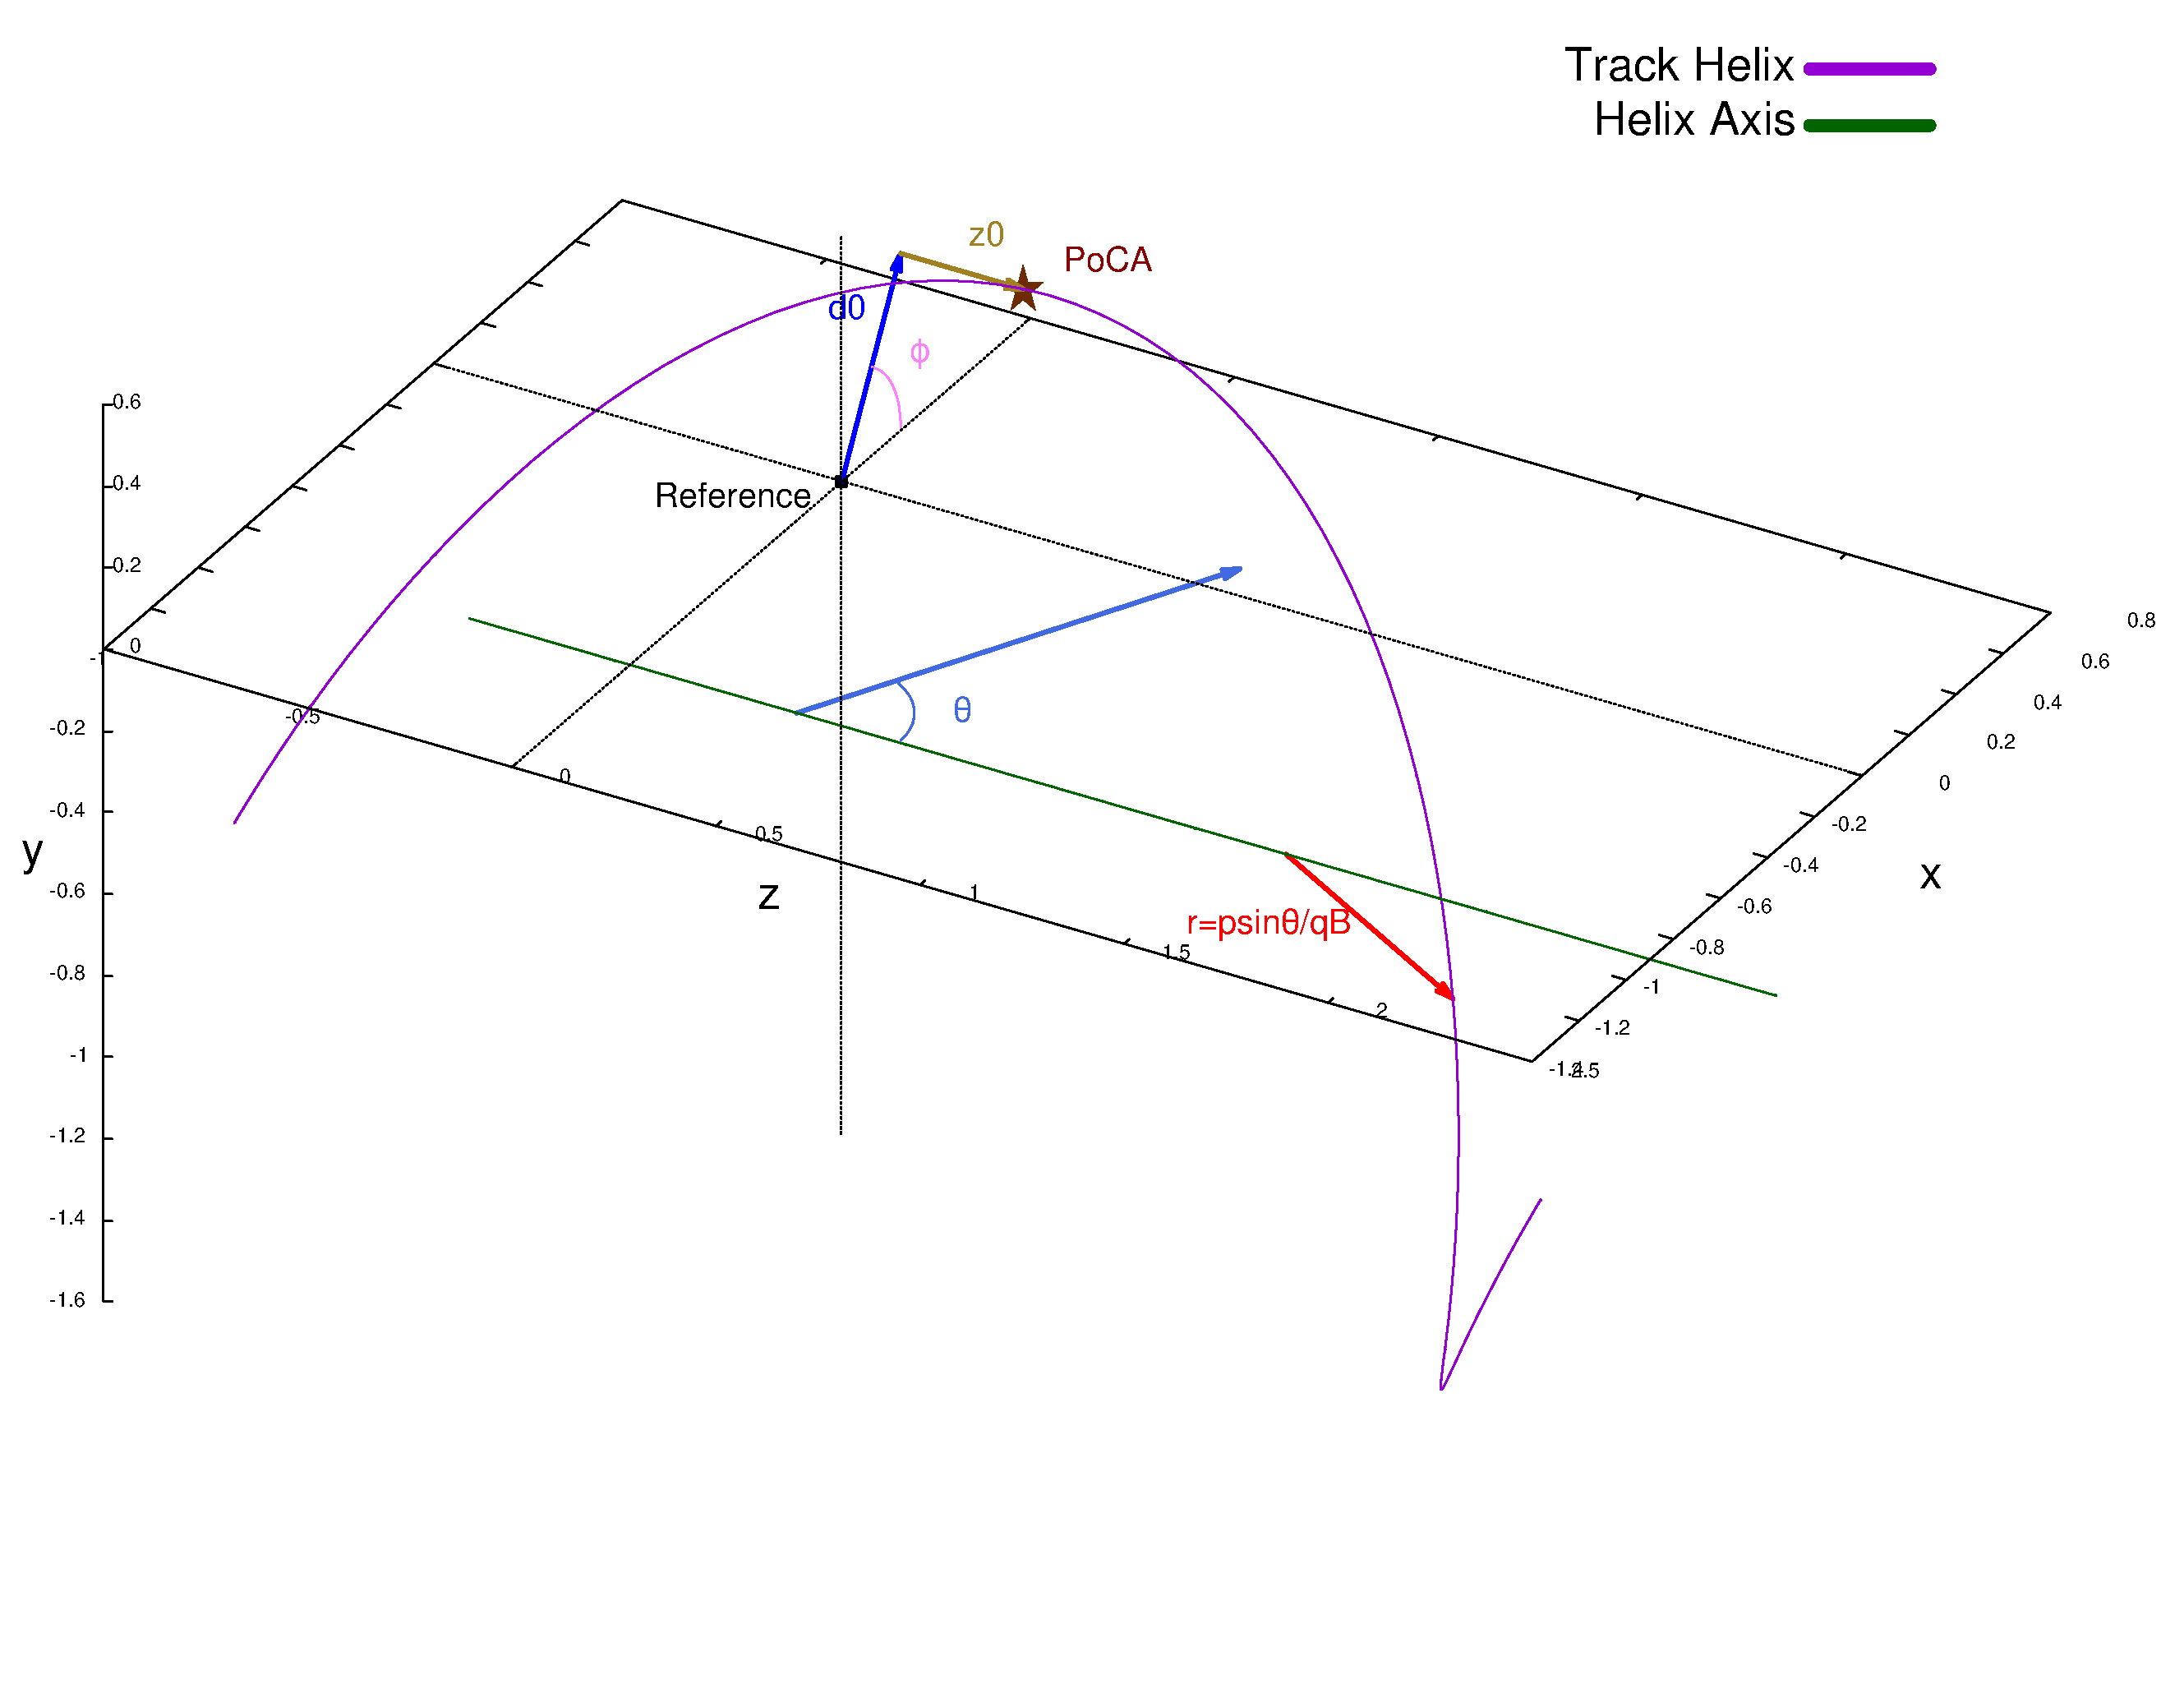
\includegraphics[width=0.5\linewidth,height=\textheight,keepaspectratio]{reconstruction/perigee_base}
                }
                \subfloat[Front View, $(x,y)$-Plane]{
                    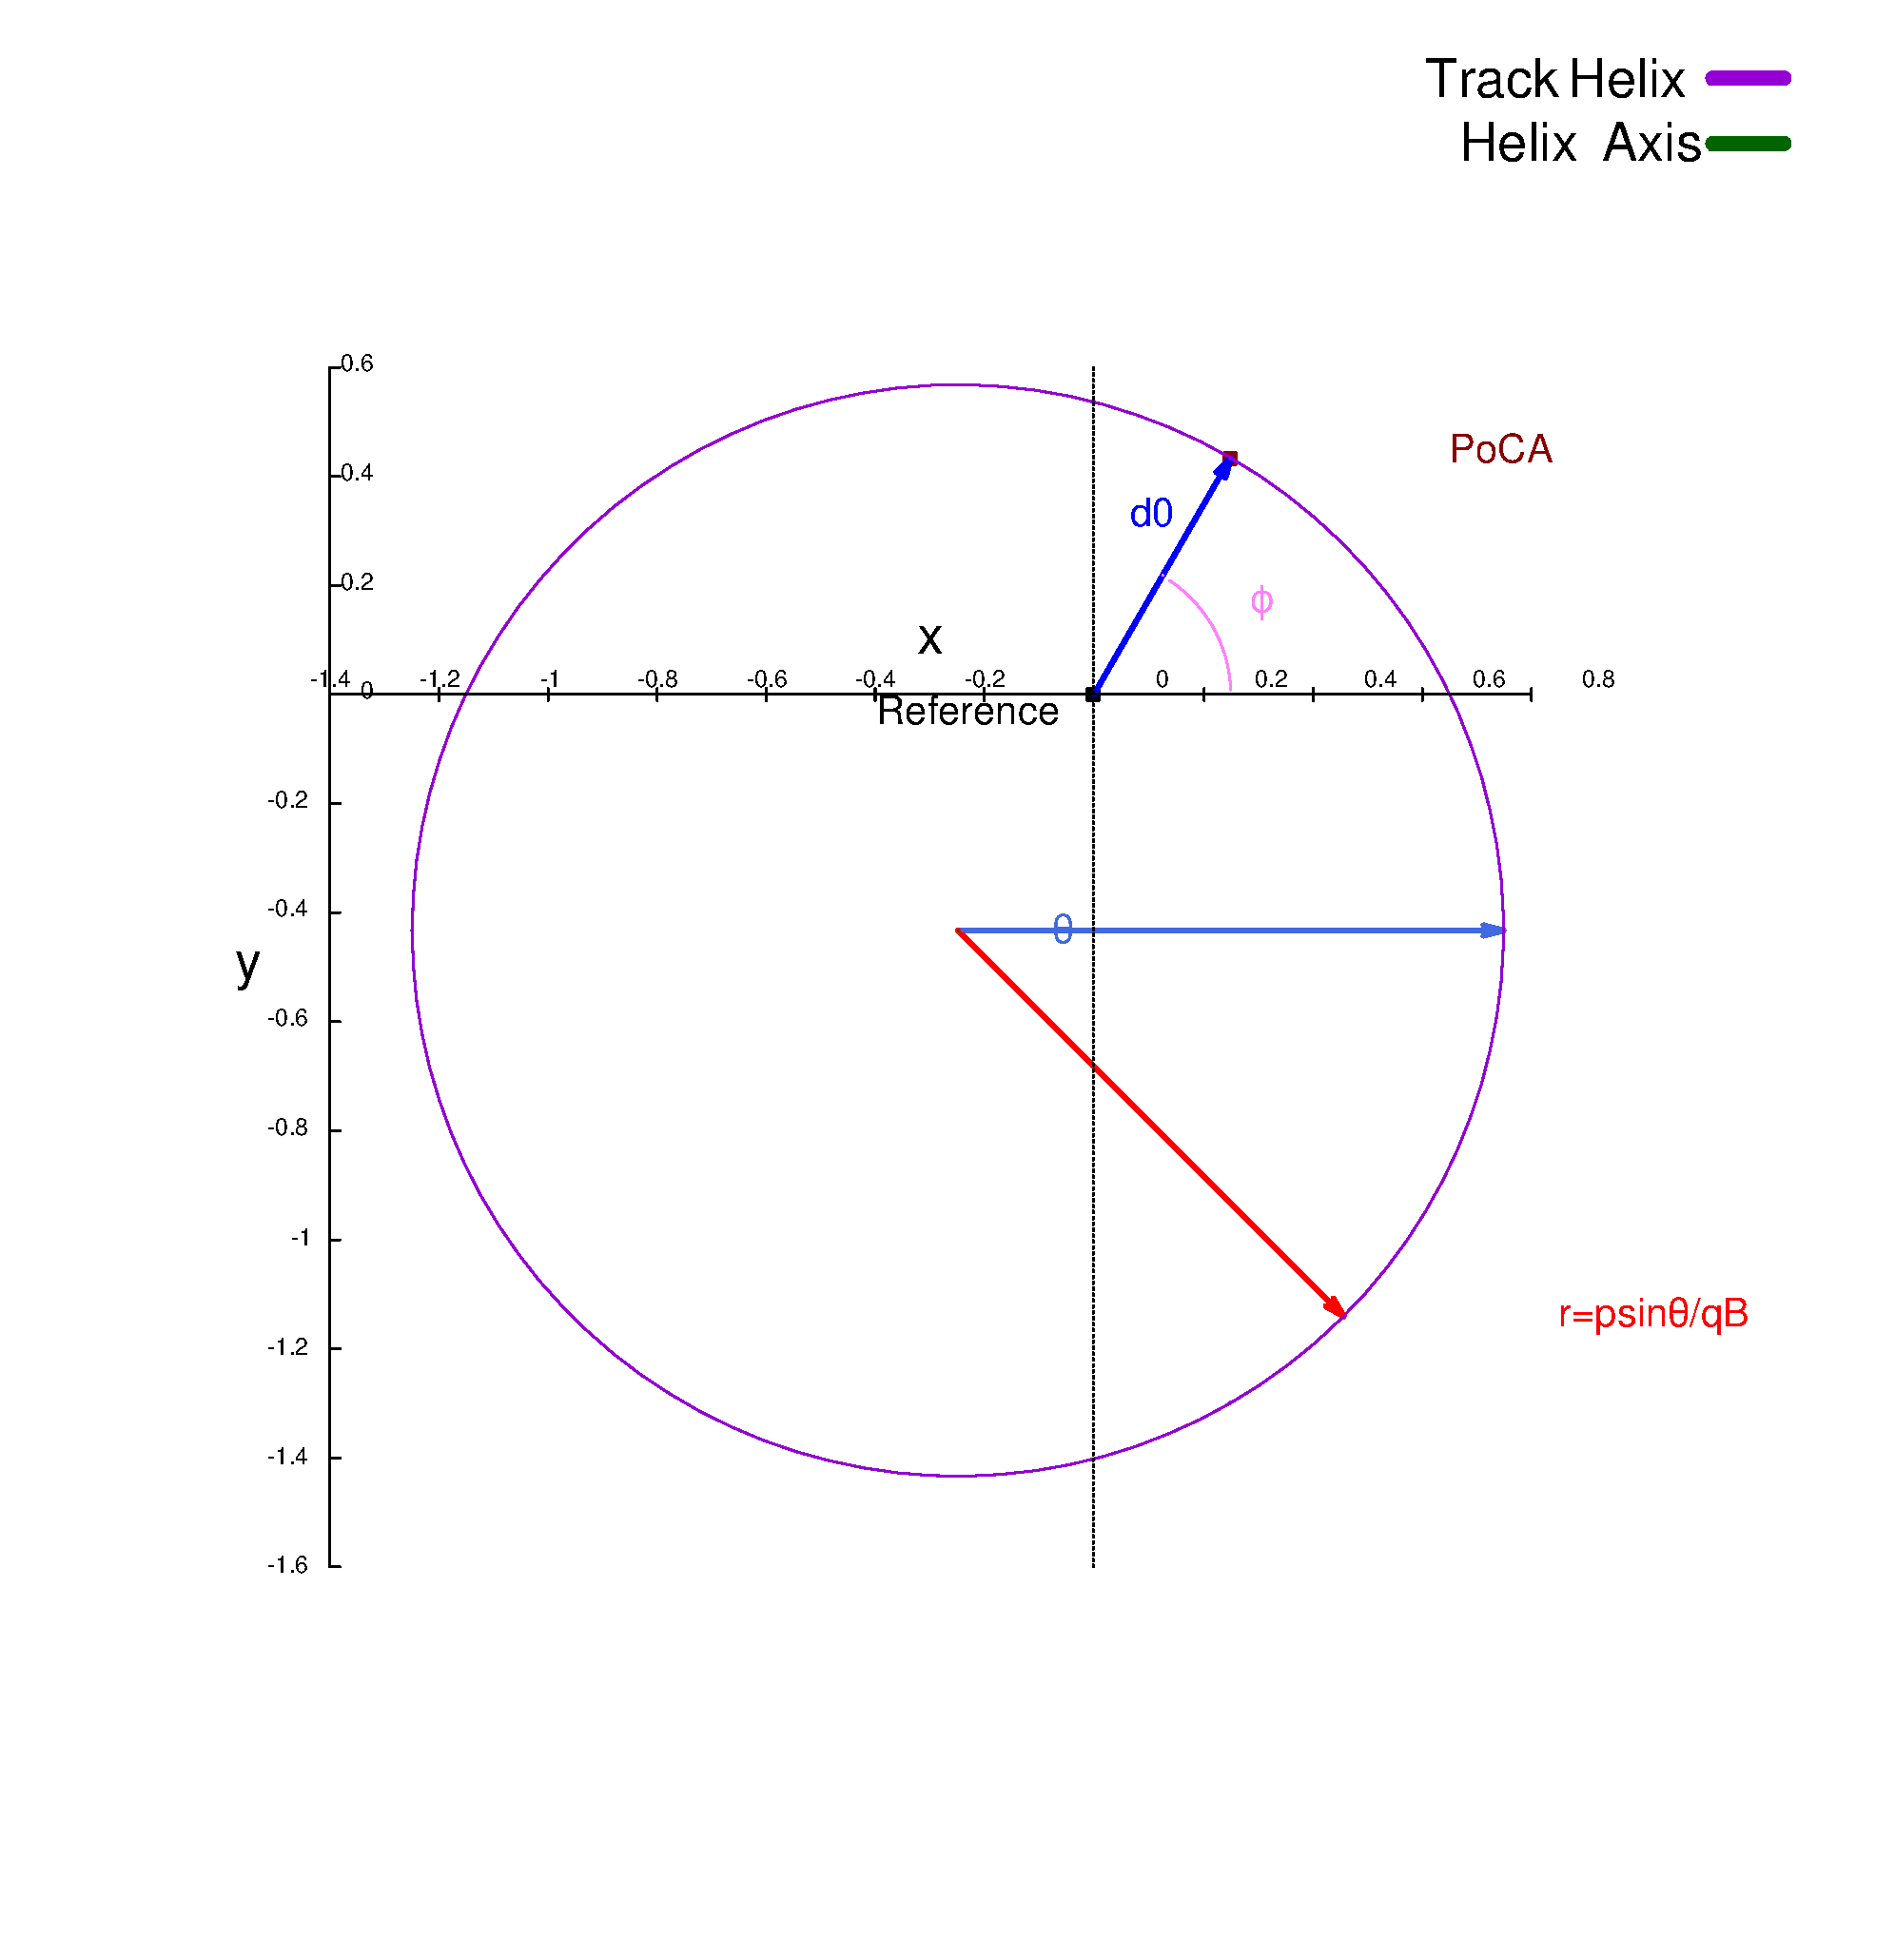
\includegraphics[width=0.5\linewidth,height=\textheight,keepaspectratio]{reconstruction/perigee_front}
                }\\
                \subfloat[Top View, $(x,z)$-Plane]{
                    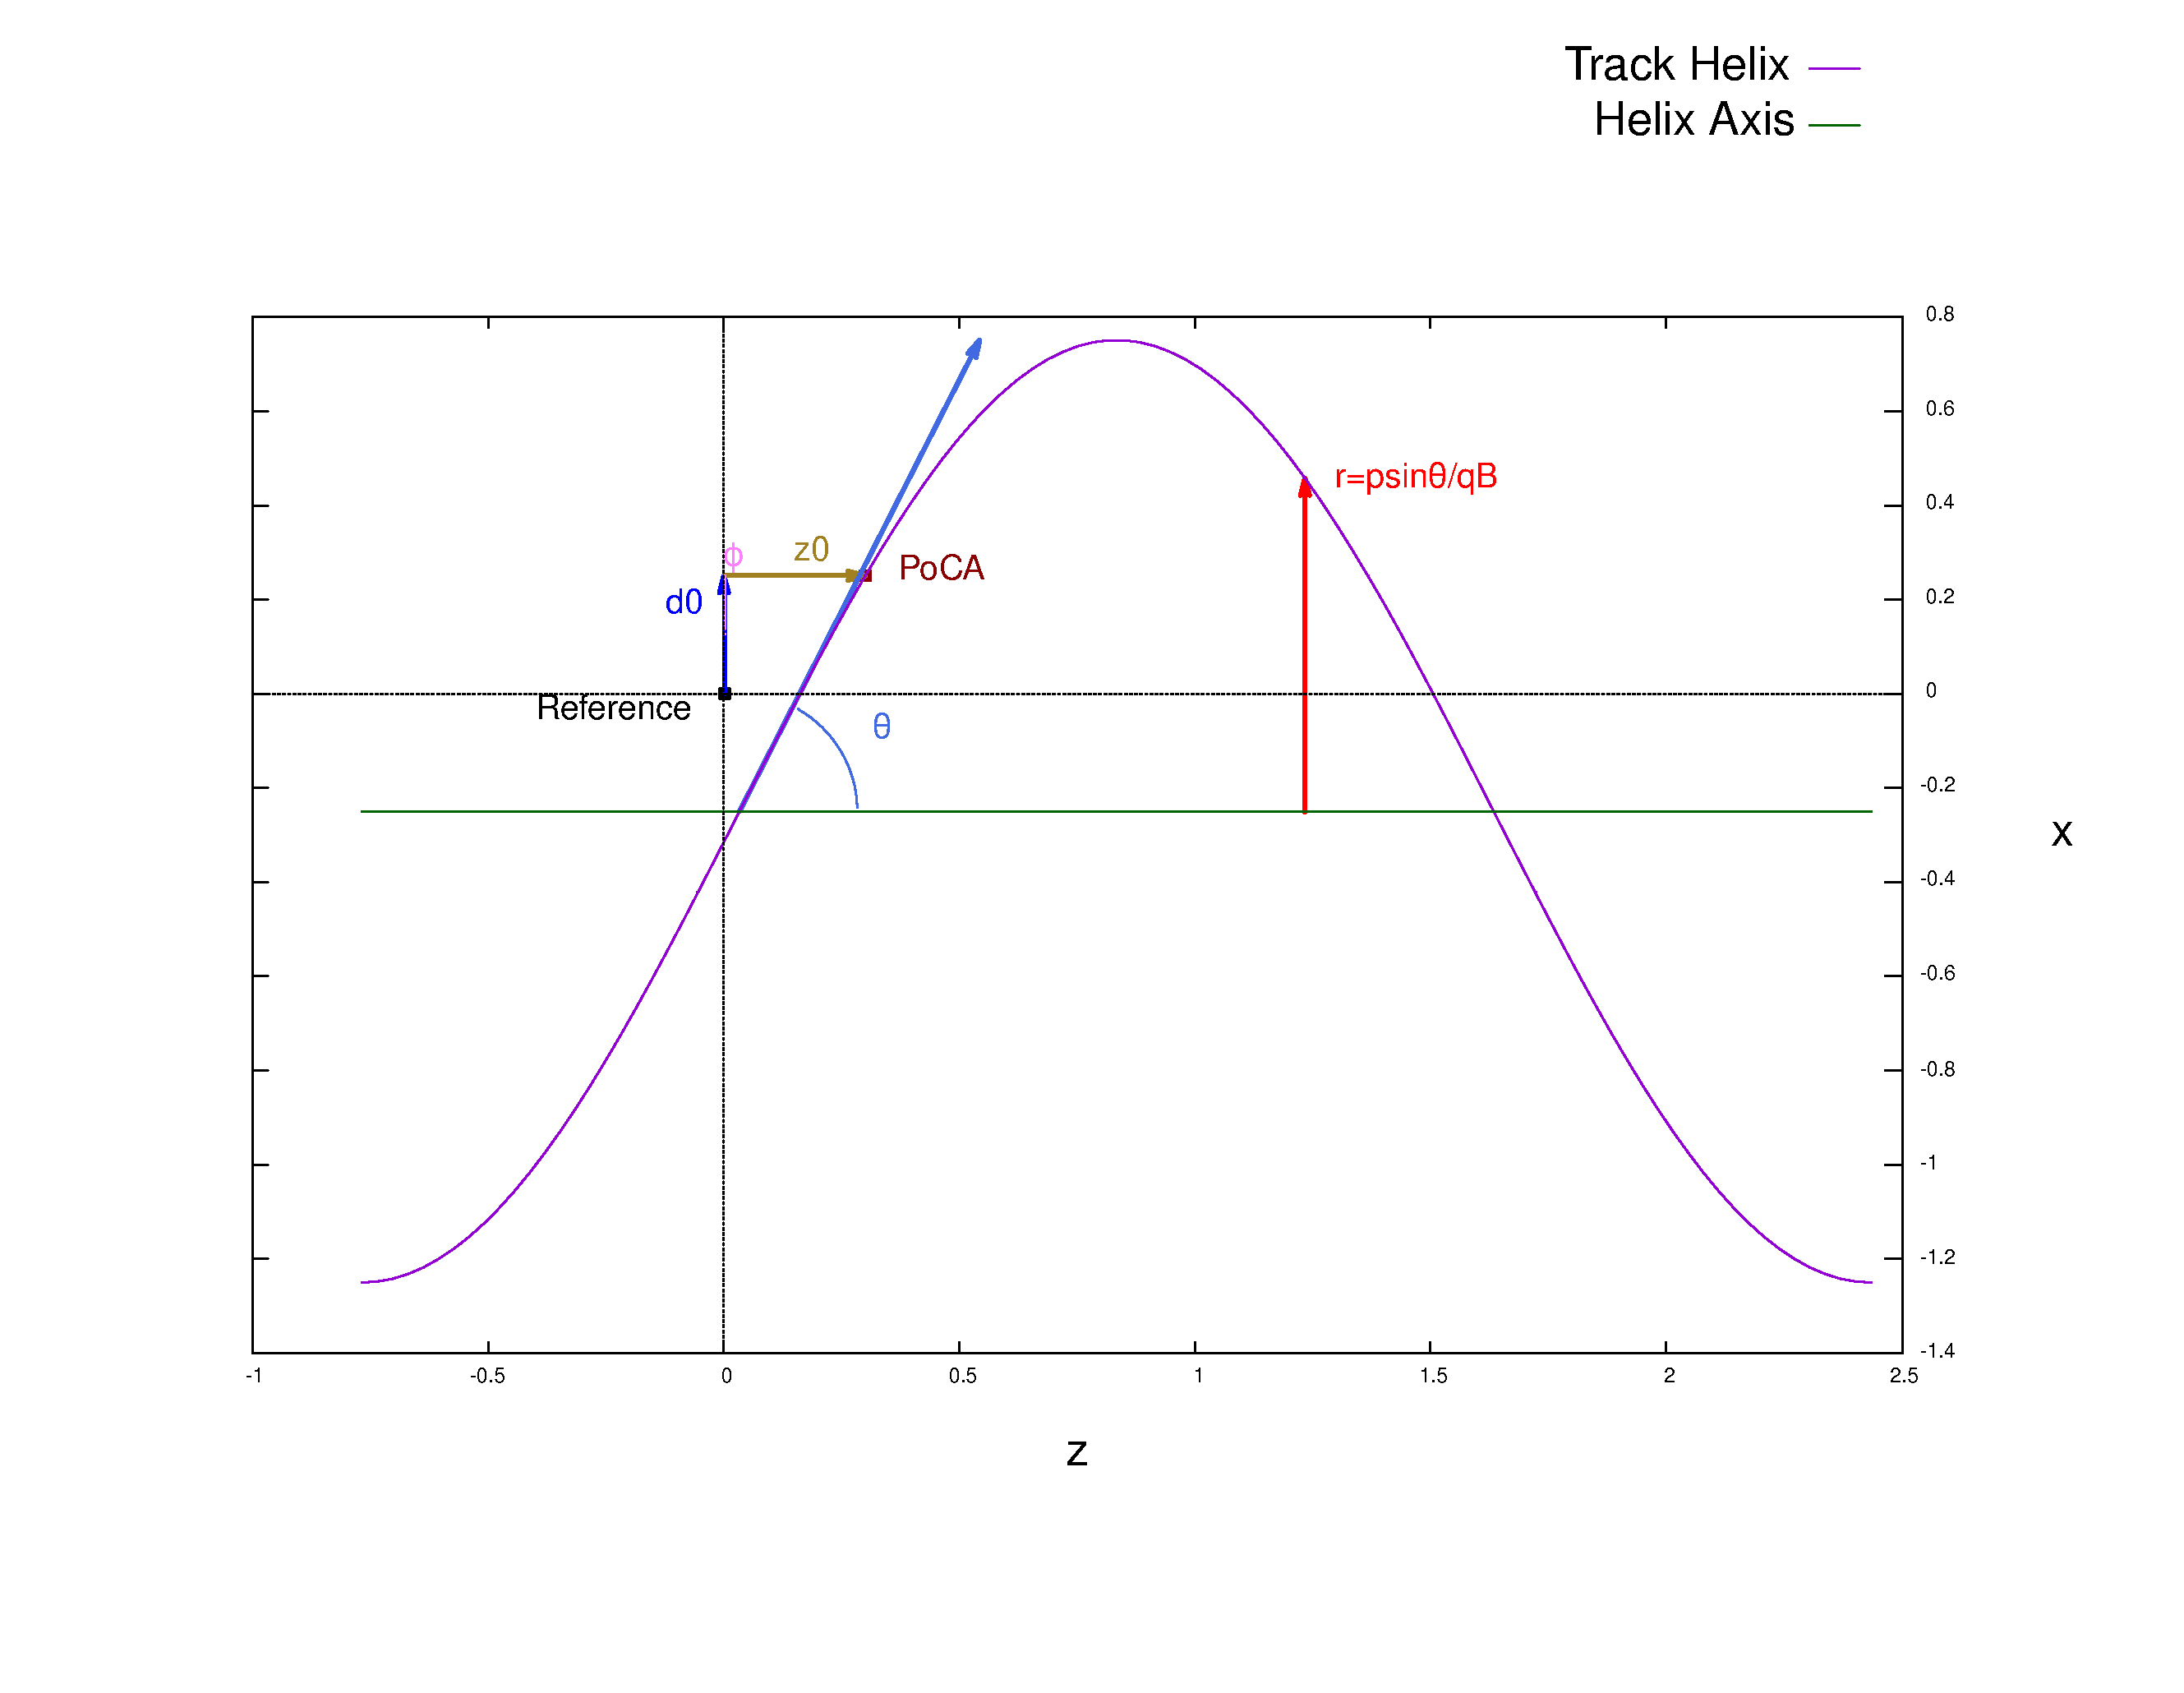
\includegraphics[width=0.5\linewidth,height=\textheight,keepaspectratio]{reconstruction/perigee_top}
                }
                \caption{
                    A diagram showing a helix trajectory from multiple angles,
                        with the five perigee parameters highlighted.
                    [FIXME: Perigee parameters are hard!
                    Also I need to replace PV with just `Reference', since the PV comes later (oops).
                    Also I should make the labels on these bigger.]
                }
                \label{fig:perigee_params}
            \end{figure}

            All five of the parameters are used at some stage of the analysis.
            With regards to the aformentioned particle momentum, $\phi$ and $\theta$ are themselves components of the particle's 4-vector.
            $\rho$ can then be related to the particle's transverse momentum and electric charge as
            \begin{equation}
            r = \frac{p_T}{qB} = \frac{|\vec{p}| \sin(\theta)}{qB}
            \end{equation}
            where $B$ is the magnetic field of the Inner Detector Solenoid Magnet\cite{thesis_track_sim_and_reco}.
            Note that uncharged particles, like photons, will not be bent, and will thus have no curvature,
                negating the ability to measure their transverse momentum in this way.
            The impact parameters, $d_0$ and $z_0$, are not related to momentum,
                but will be used in later sections for the purpose of flavour tagging.

        \FloatBarrier
        \subsection{Track Reconstruction}

            As particles pass through the inner detector subsystems, they trace out a path of ionized detector elements.
            This trajectory can be reconstructed by effectively playing connect-the-dots.

            %Clusterization
            The first step in reconstructing a track is to determine where the dots to connect actually are, 
                a process called ``clusterization''.
            Ionizing particles often deposit energy across several adjacent pixels on a given layer.
            A \textit{connected component analysis} algorithm is used to group pixels together.
            Based on the pattern of energy distribution in these groups,
                a \textit{space-point} (the ``dot'' in my metaphor) 
                is created indicating the estimated position at which a particle crossed the detector.
            Several space-points can be assigned to the same pixel cluster
                if the energy readout pattern suggests multiple particles traversed the same location.

            \begin{figure}[tbh]
                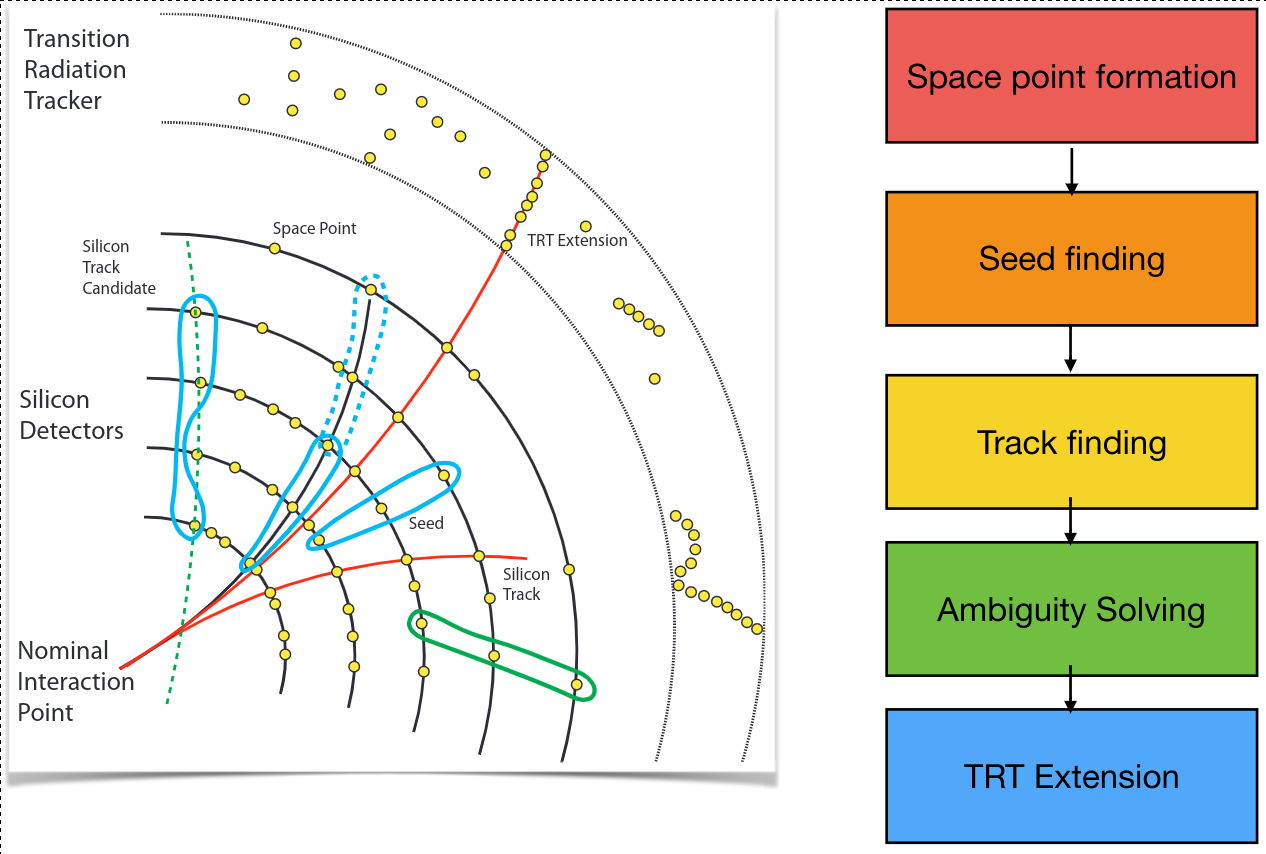
\includegraphics[width=\linewidth,height=\textheight,keepaspectratio]{reconstruction/track_reconstruction}
                \caption{
                    Diagram of track fitting in the ATLAS inner detector
                    [FIME: Steve how do I cite an indico presentation? Also is this even a good image to use?].
                }
                \label{fig:atlas_shower}
            \end{figure}

            %Combinatorial track finding
            Once the ``dots'' are established, a series of guesses at how they should be connected are made.
            Initial guesses at tracks, called track seeds, are formed by assembling all realistic combinations of three space-points.
            The track seeds are assigned helix parameters by assuming they travel through a uniform magnetic field,
                allowing rapid estimates of the tracks' momentum.
            These seeds are expanded into \textit{track candidates},
                by including more space-points across additional detectors in the ID using a \textit{Kalman filter}.

            %Ambiguity solving; NN clustering; Track fit
            The last step is then to choose a final ``picture'' that looks the most valid.
            A number of criteria are used to reject poor-quality tracks, as well as to assign scores to all remaining track candidates.
            These scores are used to resolve ambiguities where multiple tracks are assigned to the same space-points,
                with preference given to higher-scoring candidates.
            Neural networks are used to assist in some ambiguity solving situations,
                as well as to help identify clusters with multiple valid tracks.
            Once ambiguities have been resolved and all malformed track candidates removed,
                the remaining tracks are refit using all available information at high-resolution\cite{atlas_track_reco_performance}.

        \FloatBarrier
        \subsection{Primary Vertexing}

            Once track filtering has concluded,
                the remaining tracks can be used to identify a key piece of event information, 
                called the \textit{Primary Vertex}.
            When bunches collide in the IR of ATLAS, most of the collisions of a given bunch are fairly minor.
            Events which clear the L1 trigger however, typically do so because of the presence of a hard-scatter interaction. %FIXME: really?
            Identifying the location along the beamline at which this hard-scatter interaction occurred is achieved via ``vertex-finding.''
            Points along $z$ from which particles originate are referred to as ``vertices''.
            They are identified in reconstruction by tracing the reconstructed tracks backwards
                and identifying points at which they intersect the $z$-axis.
            All tracks which intersect at the same point are associated to that vertex.
            Most of the vertices are of little interest, and are known as Pile-up vertices.
            The vertex assumed to be the location of the hard-scatter interaction, called the Primary Vertex (PV),
                is identified as a vertex associated with at least two tracks,
                and whose tracks posses the largest sum of squared momentum\cite{jet_energy_scale13TeV}.
            Once the primary vertex is identified, the high resolution track fitting step is rerun,
                but now with the PV set as the reference point $R$ instead of the beamspot.


    \FloatBarrier
    \section{Jets}

        \subsection{Jet Definition}

        Moving outwards from the inner tracker into the calorimeters, focus shifts from tracks to the reconstructed objects known as \textit{jets}.
        Jets are an attempt to encapsulate the process of scattering within high-Z materials.
        A high energy particle encountering the heavy-metal plates in the calorimeters will be deflected,
            while releasing other particles which travel in different directions.
        All these new particles will produce similar reactions, until the various particles posses too little energy to cause further scattering.
        The overall effect appears as a roughly cone-shaped shower of particles,
            whose ``tip'' is located somewhere near the interaction vertex.
        This cone has an associated vector corresponding to the direction the cone opens out at.
        Due to conservation of momentum, the momentum vector of the original particle will be roughly equal to the jet vector,
            since the total momentum of the various scattered particles must sum back to the momentum of the initial particle.

        \begin{figure}[tbh]
            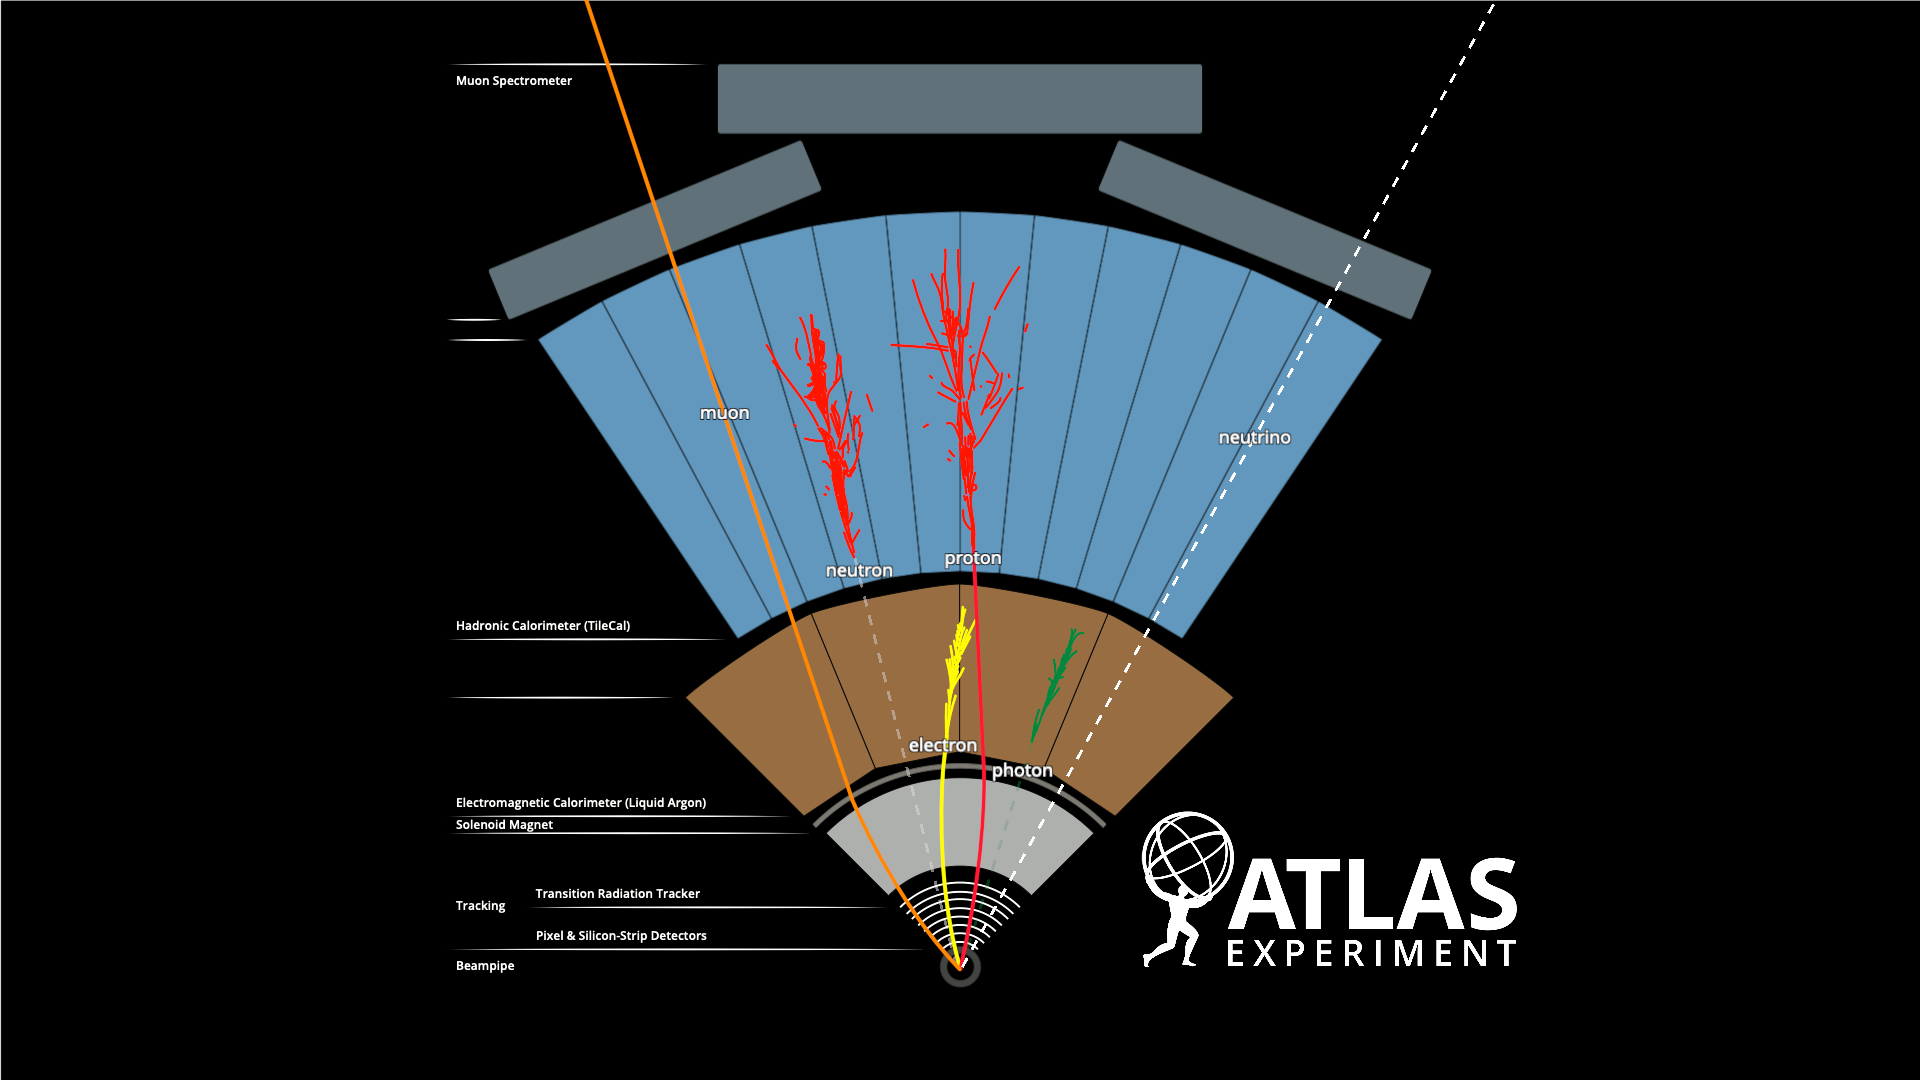
\includegraphics[width=\linewidth,height=\textheight,keepaspectratio]{reconstruction/ATLAS_Detector_Schematic_black_particles}
            \caption{
                Depiction of different particle types showering through the ATLAS detectors\cite{Mehlhase:2770815}.
            }
            \label{fig:atlas_shower}
        \end{figure}

        Though jets are meant to represent a physical phenomenon,
            it should be emphasized that jets themselves \textit{are not physical objects}.
        Rather, jets are an algorithm.
        Specifically, jets are an algorithm used to cluster different cells in a calorimeter together,
            based on the energy deposited in each cell.
        The general goal is to have each complete ``topological cluster'' (topo-cluster) correspond to one particle.
        In practice however, particles frequently overlap in their energy deposition,
            making it challenging to distinguish where one cluster should begin and another should end.
        Historically, a number of different jet algorithms have been used to describe particle showers.
        In ATLAS, the jet algorithm currently in use is the \textit{\antikt} clustering algorithm\cite{anti_kt}.
        Adoption of \antikt has been motivated by its robust ability to isolate jet boundaries both from each other,
            and from the surrounding stochastic noise of the detector.
        The \antikt algorithm has a single input parameter ``$\Delta R$'' which roughly corresponds to the ``radius''
            of the jets that \antikt should attempt to match to.
        %what is delta R
        This radius is a solid angle (in $\phi$ and $\eta$) distance from the center of the topo-cluster,
            such that $\Delta R^2 \equiv \Delta \eta^2 + \Delta \phi^2$.
        A $\Delta R$ value of 0.4 is the standard for jets in ATLAS, and is used for this analysis.
        This value means that \antikt will generally keep aggregating cells together until the topo-cluster's
            $\Delta R$ radius equals 0.4, and not much beyond that.
        [NOTE: Hey Steve, do I need to describe how antikt works?
        It's not that complicated, but it's kinda weird and unintuitive and I'm not sure if its description would add much]

        \FloatBarrier
        \subsection{Jet Calibration}

        Once topo-clusters have been formed, their energy and momentum must be calibrated.
        As discussed in Section \ref{sec:calorimeter}, the ATLAS calorimeters are sampling calorimeters.
        This means that the bulk of energy deposited is lost in inactive material, and not read out.
        Additional energy losses are incurred from inefficiencies in the clustering algorithm and from the \textit{non-compensating} nature of ATLAS calorimeters.
        That is, they do not have an intrinsic method to account for the fact that electromagnetic radiation deposits a higher fraction of its energy into the detectors than hadronic radiation\cite{cell_clustering}.

        After correcting for energy, the next step is to correct for momentum.
        Reconstructed jets are assumed to originate from the hard-scatter interaction point.
        Thus, the momentum vectors associated with the jets and their topo-clusters are adjusted to point away from the PV.

        The final step in the jet reconstruction process is the track-matching algorithm.
        To improve the performance of reconstructing hadronic jets
            the various jet vectors are each matched to a corresponding track that the jet likely started from.
        This algorithm, called \textit{Particle Flow}, treats the jets as extensions of the reconstructed particles,
            matching jets to tracks based on both location and energy projections.
        The resulting jet-track combination objects are known as \textit{PFlow Jets},
            which are then used for the rest of the reconstruction process\cite{pflow}.

        %Jets created using only calorimeter-based topological-clusters (at the electromagnetic scale [what does this mean??]) %TODO?
            %are referred to as \textit{EMtopo Jets}. %I still don't really get this, and I'm not sure they're even really used, so imma skip it

    \FloatBarrier
    \section{Flavour Tagging}
        
        There are many kinds of particles and processes that can produce jets.
        One particular kind of jet integral to this analysis is that of b-quark-initiated jets,
            more simply known as b-jets.
        B-jets are important because, of all the particles the Higgs can decay to,
            its branching ratio to a $\bbar$ pair is highest.
        Distinguishing b-jets from other jet types,
            achieved through the process of \textit{flavour tagging},
            is therefore of paramount importance in this analysis.
        Flavour Tagging in ATLAS is performed in two stages;
            first with a set of simple low-level taggers,
            and then with a set of more sophisticated taggers which use the low-level tagger information as inputs.

        TODO: insert table of branching fraction of higgs? Should that go here or elsewhere?

        \FloatBarrier
        \subsection{Impact Parameter Taggers}

            The low-level b-tagging algorithms can be divided between impact parameter taggers and secondary vertexing algorithms.
            IP2D and IP3D are the two and three-dimensional impact parameter-based taggers.
            They take every track associated with a PFlow Jet,
                and then use a slightly modified version of the perigee parameters discussed above in order to tag it.
            Namely, the $d_0$ and $z_0$ parameters are given a positive or negative sign to help better emphasize key characteristics of b-jets\cite{thesis_giacinto}.
            \begin{equation} \begin{split}
                \textrm{sign}_{d0} &= \textrm{sign}(\sin(\phi_{\textrm{jet}} - \phi_{\textrm{track}}) \cdot d_{0,\textrm{track}}) \\
                \textrm{sign}_{z0} &= \textrm{sign}((\eta_{\textrm{jet}} - \eta_{\textrm{track}}) \cdot z_{0,\textrm{track}})
            \end{split} \end{equation}
            Physically, this sign convention is to distinguish tracks which are likely to have actually been part of the jet (with a positive sign)
                from those likely originating from pile-up vertices (negative sign).
            [TODO: I'm not sure these equations are actually right. At the very least, I don't understand them, so I'll need to revisit this]
            See Figure \ref{fig:ip3d_sign} for a graphical illustration of this convention.

            \begin{figure}
                \subfloat[IP3D Negative Sign Convention]{
                    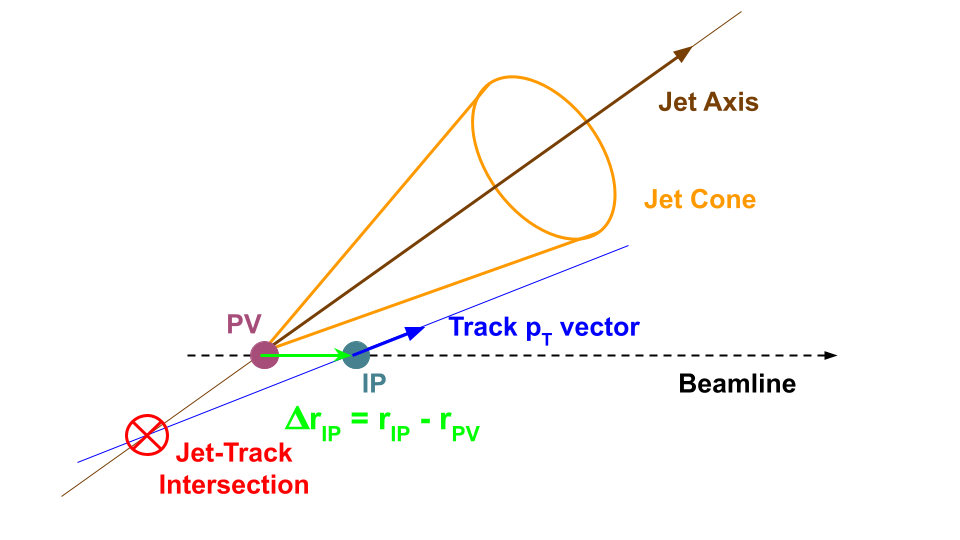
\includegraphics[width=0.5\linewidth,height=\textheight,keepaspectratio]{reconstruction/ip3d_sign_negative}
                }
                \subfloat[IP3D Positive Sign Convention]{
                    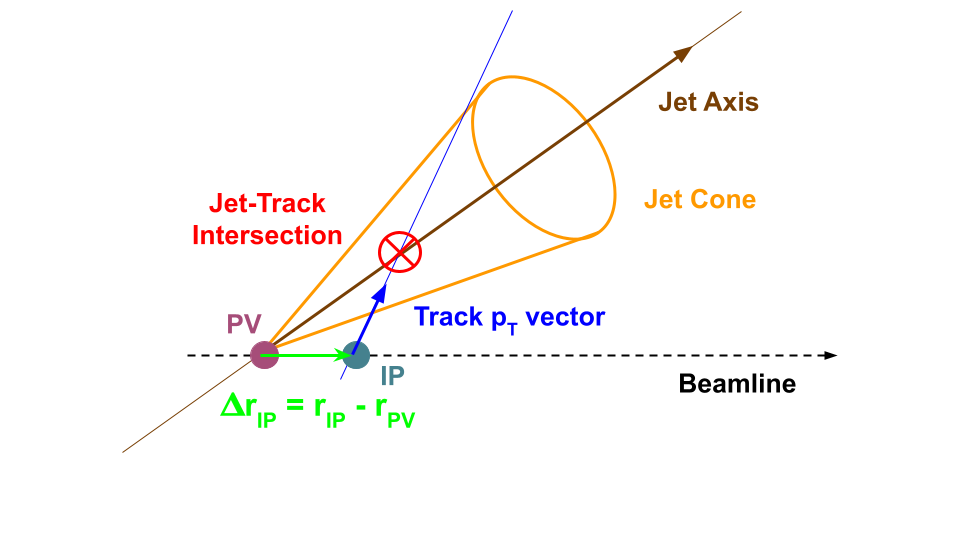
\includegraphics[width=0.5\linewidth,height=\textheight,keepaspectratio]{reconstruction/ip3d_sign_positive}
                }
                \caption{
                    Diagrams of the sign convention used for IP3D.
                    In the left diagram, the track $p_T$ vector intersects with the jet $p_T$ vector axis
                        \textit{before} the PV, suggesting this track originated from a source unrelated to the PV
                        (and is thus likely just noise from a pileup vertex).
                    In the right diagram, the track $p_T$ vector intersects with the jet $p_T$ vector axis
                        \textit{after} the PV, suggesting this track originated from a secondary vertex of
                        a particle emitted from the PV
                        (around the area marked with a red X).
                    \cite{thesis_giacinto}.
                }
                \label{fig:ip3d_sign}
            \end{figure}

            Values are assigned to \textit{each} track in a jet based on probability density functions (PDF) of the different jet types.
            Specifically, a PDF is constructed of the impact parameter \textit{significance}, $d_0/\sigma_{d0}$,
                where $\sigma_{d0}$ is the error of the measurement.
            The probability that a given track, $i$, would have some impact parameter significance value (based on the PDF)
                is that track's assigned IP2D value, $t_i$.
            IP2D and IP3D are then constructed as likelihood ratios of the product of all track-values for a jet.
            For example, the likelihood ratio of a jet being a b-jet versus a light-jet would be based on
                the PDF of the impact parameter for b-jets ($\textrm{PDF}_b$) to that for light-jets ($\textrm{PDF}_l$)

            \begin{equation}
                R(t_1, t_2, ... t_N) \equiv \frac{\prod_{i=1}^N \textrm{PDF}_b(t_i)}{\prod_{i=1}^N \textrm{PDF}_l(t_i)}
            \end{equation}

            These distributions are subsequently used as a discriminant to distinguish b-jets and charm-jets from light-jets
                (see Figure \ref{fig:ip3dsig})\cite{thesis_giacinto}. %TODO: is there a non-empirical, like, physics reason for this?

            \begin{figure}
                \subfloat[IP3D-$d_0$, 2016]{
                    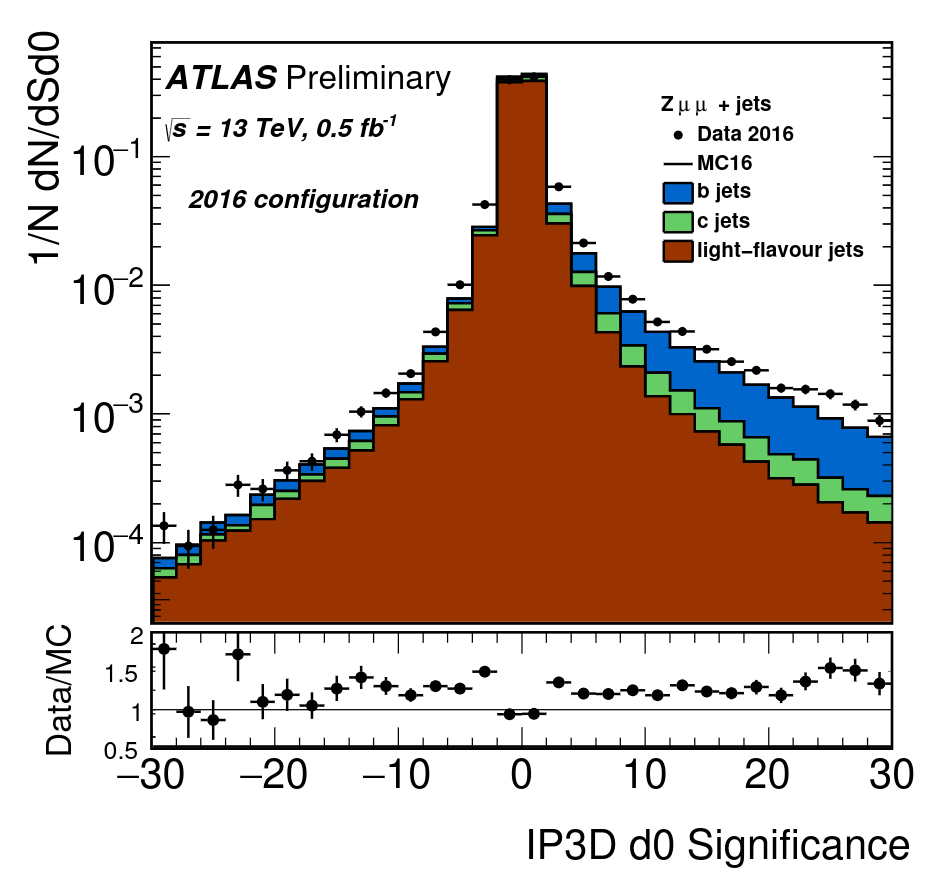
\includegraphics[width=0.5\linewidth,height=\textheight,keepaspectratio]{reconstruction/ip3d_d0_sig_2016}
                }
                \subfloat[IP3D-$d_0$, 2017]{
                    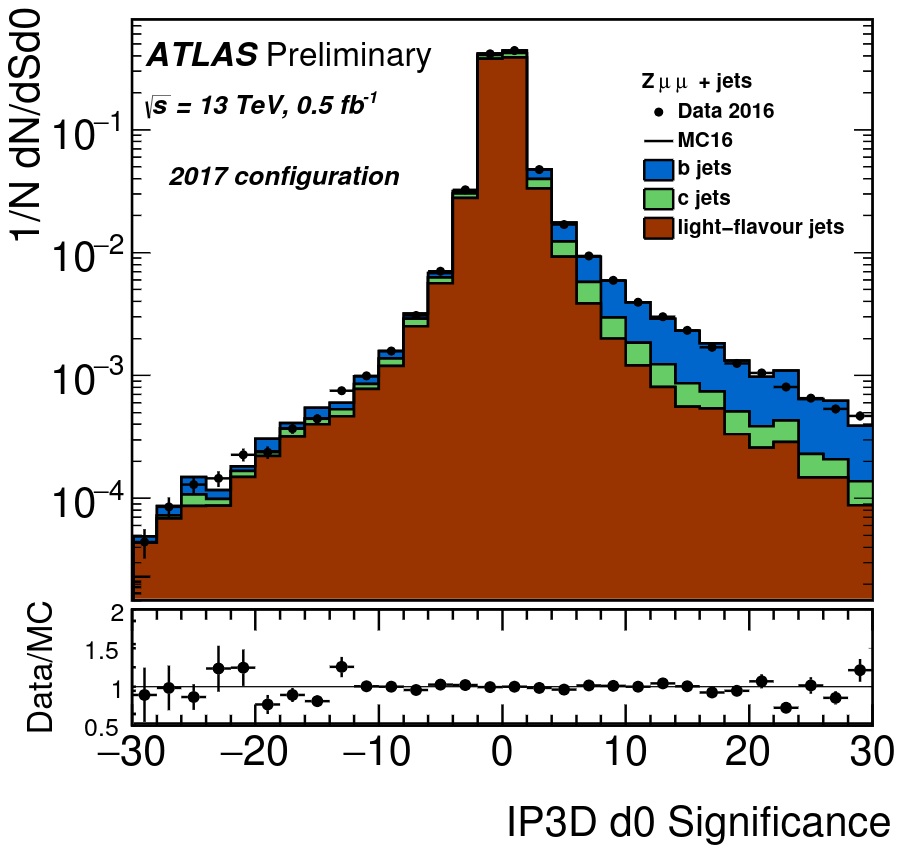
\includegraphics[width=0.5\linewidth,height=\textheight,keepaspectratio]{reconstruction/ip3d_d0_sig_2017}
                }\\
                \subfloat[IP3D-$z_0$, 2016]{
                    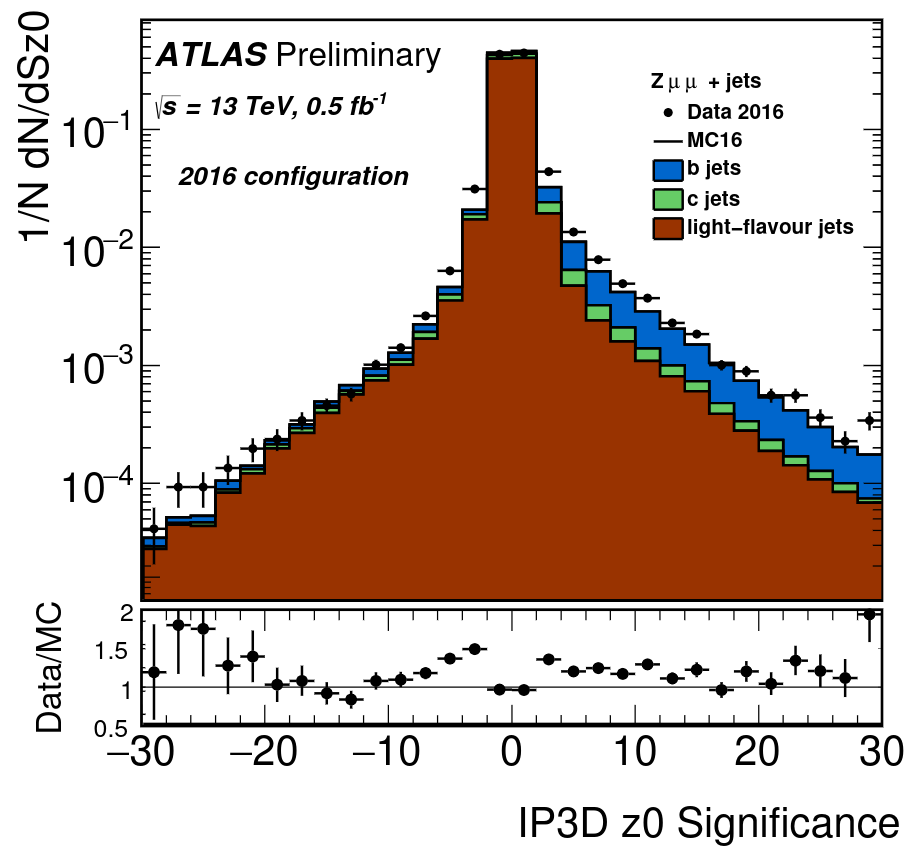
\includegraphics[width=0.5\linewidth,height=\textheight,keepaspectratio]{reconstruction/ip3d_z0_sig_2016}
                }
                \subfloat[IP3D-$z_0$, 2017]{
                    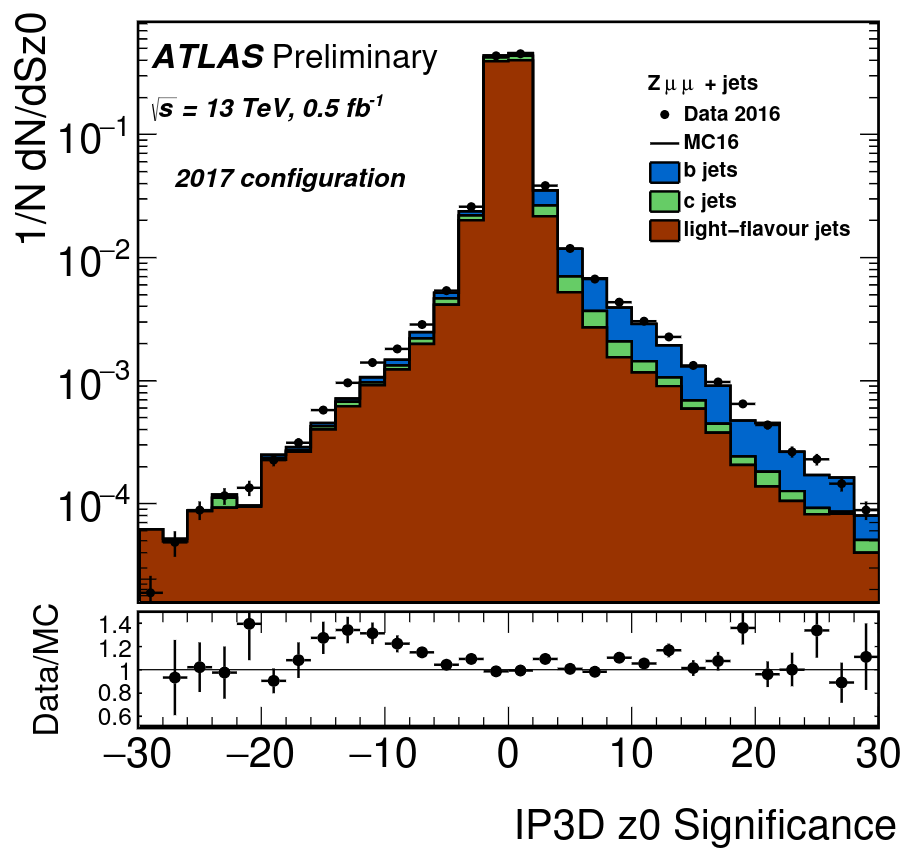
\includegraphics[width=0.5\linewidth,height=\textheight,keepaspectratio]{reconstruction/ip3d_z0_sig_2017}
                }
                \caption{
                    IP3D d0 and z0, for 2016 and 2017 configurations\cite{btagging_optimisation}.
                }
                \label{fig:ip3dsig}
            \end{figure}


        \FloatBarrier
        \subsection{Secondary Vertexing}

            Secondary Vertexing algorithms take advantage of the fact that b-quarks are significantly longer lived than light and charm quarks,
                and thus their associated secondary vertices typically have a larger displacement from the primary vertex.
            In ATLAS, there are two primary algorithms used to perform btagging with Secondary Vertexing.
            Realistically, hadronic matter decays in multiple steps, producing a series of close vertices each emitting more particles.
            The first of the ATLAS Secondary Vertex algorithms, JetFitter, seeks to reconstruct this full multi-vertex structure of the hadronic decay.
            In contrast, SV1 (Secondary Vertex 1), works by making an approximation as to how hadronic decays behave.
            SV1 takes a simpler view of the decay process, and reconstructs all the resulting tracks as products of a single secondary vertex.
            For both algorithms, several fit parameters are produced from the vertexing,
                which are then used both as discriminant themselves,
                as well as utilized in the next step as inputs to the more advanced taggers\cite{btagging_optimisation}.

        \FloatBarrier
        \subsection{High Level Taggers}

            After running all of the low level taggers,
                the final step in flavour tagging is the use of a pair of high-level machine-learning-based tagging algorithms.
            There are two high level taggers, both trained and run using inputs from the various low-level taggers discussed earlier.
            MV2, the Multi-Variate tagger, is a boosted decision tree (BDT).
            DL1, the Deep Learning tagger, is a multi-layer neural network.
            In the case of this analysis, a recurrent neural network version of DL1, called DL1r, is used instead.
            \cite{bjet_id_and_performance}
            \cite{btagging_optimisation}
            [NOTE: This feels way too short, but I'm not sure what else to say about them... Steve?]

    \FloatBarrier
    \section{Online VS Offline Reconstruction}

        Reconstruction is actually performed for an event twice.
        It is first done rapidly, using coarse measurements and calculations,
            for the purpose of allowing the aforementioned HLT to trigger events for readout.
        These events which pass the trigger are passed off to a massive global computer cluster, called the CERN GRID.
        No longer bound by the stringent time constraints of the online running environment,
            the GRID is able to devote vast amounts of time and computing power to a second, 
            more comprehensive, reconstruction of each event.
        For both the online (HLT) and offline (GRID) environments, event reconstruction is carried out by the same suite of software,
            called \textit{Athena}.
        The main difference in how they operate is the time they can devote to calculations, especially in the context of tracking.
        As seen is Section \ref{sec:reco_tracks}, track reconstruction is very computationally intensive.
        There are many steps, and the fitting itself is a lengthy process.
        Thus, the online environment runs a slimmed-down version of the track fitting.
        This allows the HLT to reconstruct tracks much faster, but at the expense of precision and accuracy.

        Such accuracy loss in tracking has significant downstream consequences across all aspects of reconstruction.
        Of note for this analysis are the effects on flavour tagging.
        The low level flavour-taggers function on probability distributions of the parameters of the reconstructed tracks.
        With the degradation in track quality of the online environment, the PDFs of the low level taggers are altered.
        Since the low-level taggers are affected, the high-level taggers are also affected.
        To account for this, the flavour tagging algorithms undergo a \textit{retuning} procedure, 
            which adjusts how the algorithms expect tracks to look.

        The retuning process operates in five steps.
        %Step1.1 - Run HLT reco on MC files;
        First, the HLT-tuned Athena framework is run on a large sample of simulation-based data,
            which emulates the reconstruction behavior of Athena in the online environment.
        %Step1.2 - Return low level taggers on MC HLT reco;
        Based on this simulated reconstruction, the distributions used by the low-level taggers
            (e.g.\ $d0$-significance) are recorded and turned into PDFs.
        This constitutes the retuning of the low-level taggers.
        %Step2   - Rerun HLT reco on MC, now with retuned low level tagging info;
        With the low-level taggers retuned, the Athena reconstruction is run again,
            this time recording the output of the low-level taggers themselves.
        %Step3.1 - Perform BDT training for MV2 on HLT MC reco w/ low level tags;
        The low-level tagger output is now fed as input to the training frameworks for the high-level taggers.
        For MV2, this is ROOT's TMVA, and for DL1 this is the python package Keras.
        %Step3.2 - Convert training output to usable histograms;
        Once training is complete, the output machine-learning structure is converted into a form usable by Athena,
            and the full retuning is completed.
        %Step4   - Rerun HLT reco on MC once more, to get full retuned tagging output. Use output performance to determine working points;
        At this stage, the framework is run once more, in its entirety,
            so its performance can be analyzed and any potential issues addressed.

        \begin{figure}[tbh]
            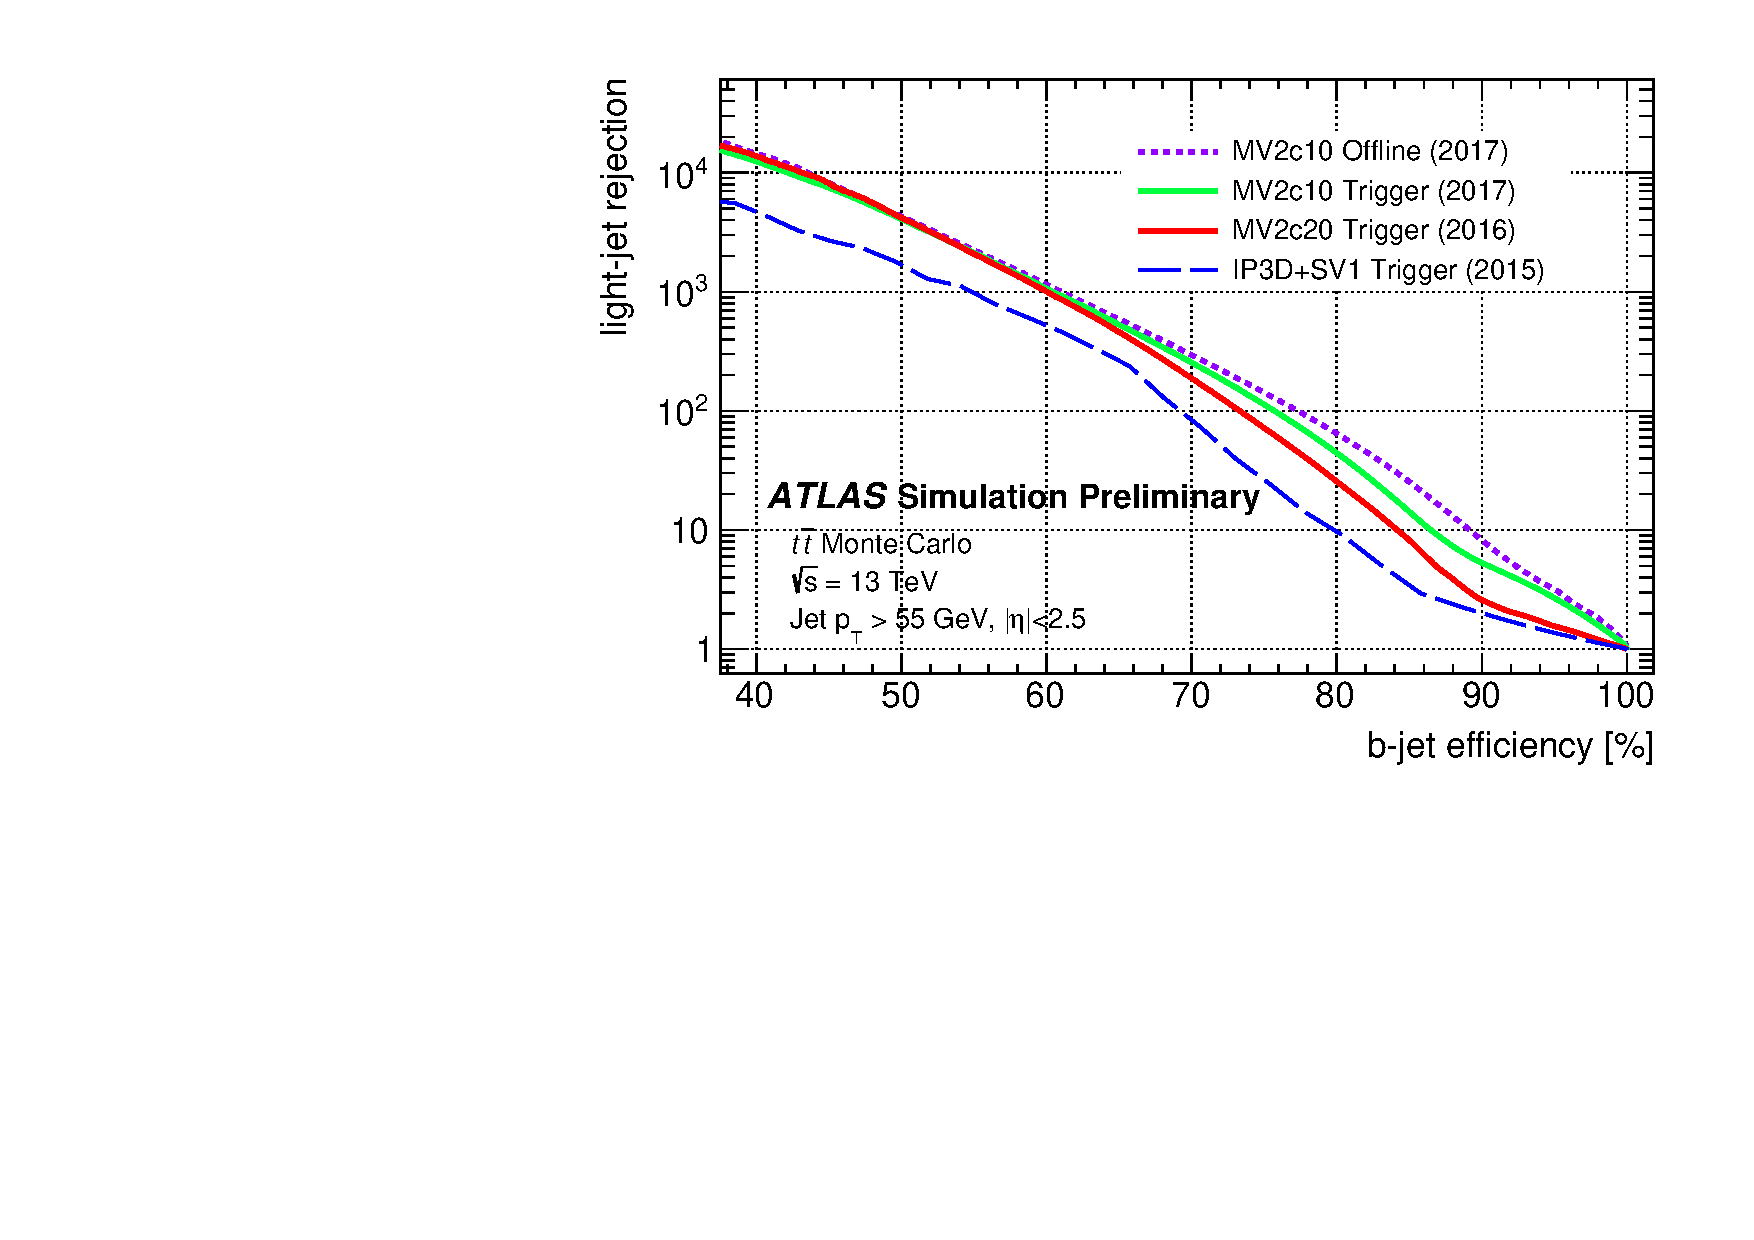
\includegraphics[width=\linewidth,height=\textheight,keepaspectratio]{reconstruction/mv2_on-off_performance}
            \caption{
                Comparison of the performance of MV2c10 and low level taggers VS offline performance\cite{Gupta:2271945}.
            }
            \label{fig:mv2_performance}
        \end{figure}

        %(We don't use mv2 for the late-stage b-tag requirement on the higgs decay candidates,
        %    but we DO use it in the triggers):

